\section{Prototypes, Sketches, Studies}

  \subsection{Studies}
  
    \subsubsection{Design Process Approach}
      \begin{figure}[H]
        \centering
        
\includegraphics[width=16cm]{prototype-1.png}
        \caption{Prototype Design Approach}
        \label{fig:design-approach}
      \end{figure}
      \par Figure \ref{fig:design-approach} shows the design process approach used to visualizing design of possible solutions. It adopted the agile development methodology similarly using the scrum technique. The UX design process was built upon 7 steps as a linear process with a sub-process of iterative and incremental cycle.
      \begin{itemize}
        \item \textbf{Step 1 – User Research}
          \par User research is a step to creating assumptions for features that are necessary and crucial for the product user. It helps to create user personas for the target audience through representations of their demographics, habits and behaviour patterns. Various data collection methods are used to collect information in an iterative breadth-and-depth approach.
        \item \textbf{Step 2 – Requirement Definition}
          \par The information collected are analysed to discover insights for involving quality features for the target audience. Hence, creating specific product requirements with documentation.
        \item \textbf{Step 3 – Sketching}
          \par Sketching helps creating in visualizing features or the product’s content to allow users to achieve their goals upon using the product. It is to provide the best possible user experience with visual components, which requires continuous feedbacks from end users.
        \item \textbf{Step 4 - Prototyping}
          \par An interactive model of the product is created with integrating suitable visual components. The prototype is made to be iterative through collecting feedbacks during usability testing.
        \item \textbf{Step 5 – Testing}
          \par Usability testing is conducted with end users consisting of probing or think-aloud techniques and A/B testing for collecting user inputs.
        \item \textbf{Step 6 – User Evaluation}
          \par Product analytics could be made with analysing and evaluate the user inputs upon the product for assessing the product potential. These inputs are studied for design and usability optimization.
        \item \textbf{Step 7 – Refining}
          \par Prototype refinement made through iterative and incremental process after user evaluation.
      \end{itemize}

  \subsection{Sketches}
  \begin{figure}[H]
    \centering
    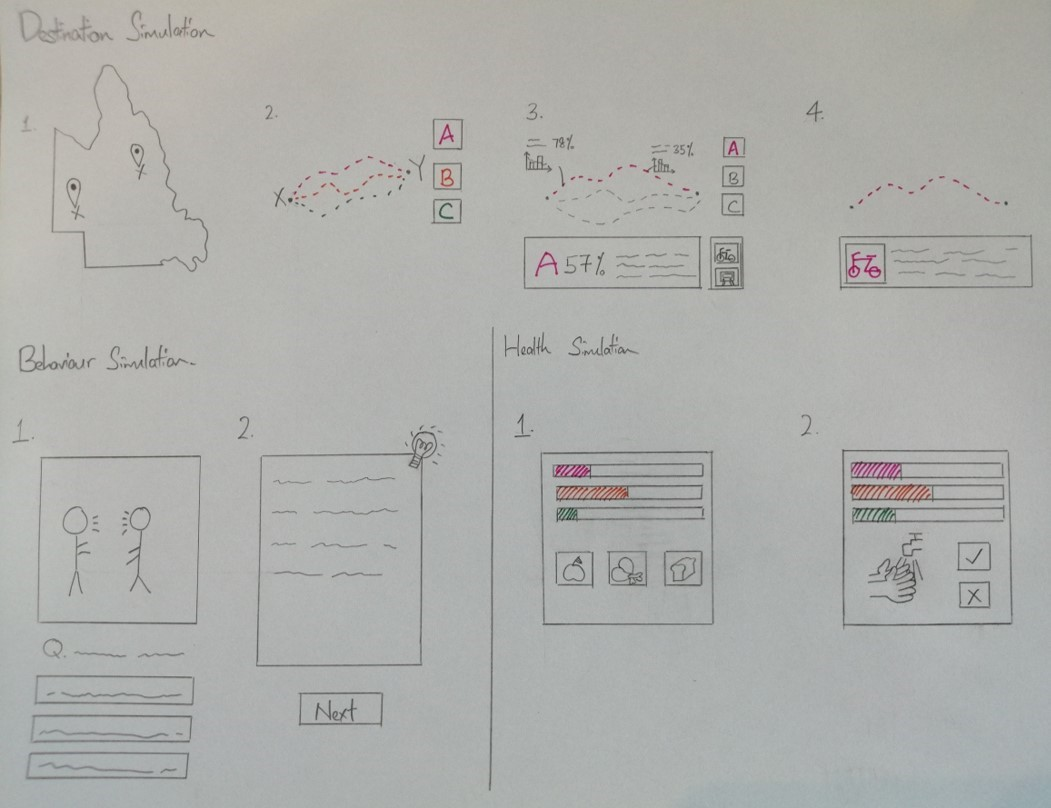
\includegraphics[width=\linewidth]{simulation.jpg}
    \caption{Simulation Sketches}
    \label{fig:simulation}
  \end{figure}
  \par Based on Figure \ref{fig:simulation}, various simulation ideas will be considered in further iterations as an implementation for the proposed solution. This provides a learning opportunity for the users, which creates interaction to achieve one of the product goals to make the platform to be more educational. Moreover, this would increase the user flow while the user interacting with the simulation, which creates possibility of more user scenarios in a simulated environment with real-life aspects during pandemic outbreak. Moreover, it could provide a pleasant user experience when information is conveyed via gamification with audio and visual components. Moreover, users could understand the value the application is trying to convey. Hence, simulation could navigate user through a journey that is projected with real-word aspects for embedding and implicit impressions for turning into habits and practices. In other words, it encourages habit and behaviour change when appropriate information is conveyed in an interactive manner be instilled into users under these special circumstances.

  \subsection{Prototypes}
    \subsubsection{Constrained Prototyping}
      \par Business Model Canvas is a method for constrained prototyping. The aim of a business model canvas is to explicit the values of the product through aligning various key elements during design planning phase. It provides a clear information outline for creating wireframe elements. Furthermore, it helps to visualize the conceptual idea of delivering a minimum viable product (MVP) which could serve as the basic form for the prototype.

      \par The canvas shown below in Figure \ref{fig:bmc} defines the general scope with descriptive points within the key elements section.

      \begin{figure}[H]
        \centering
        % 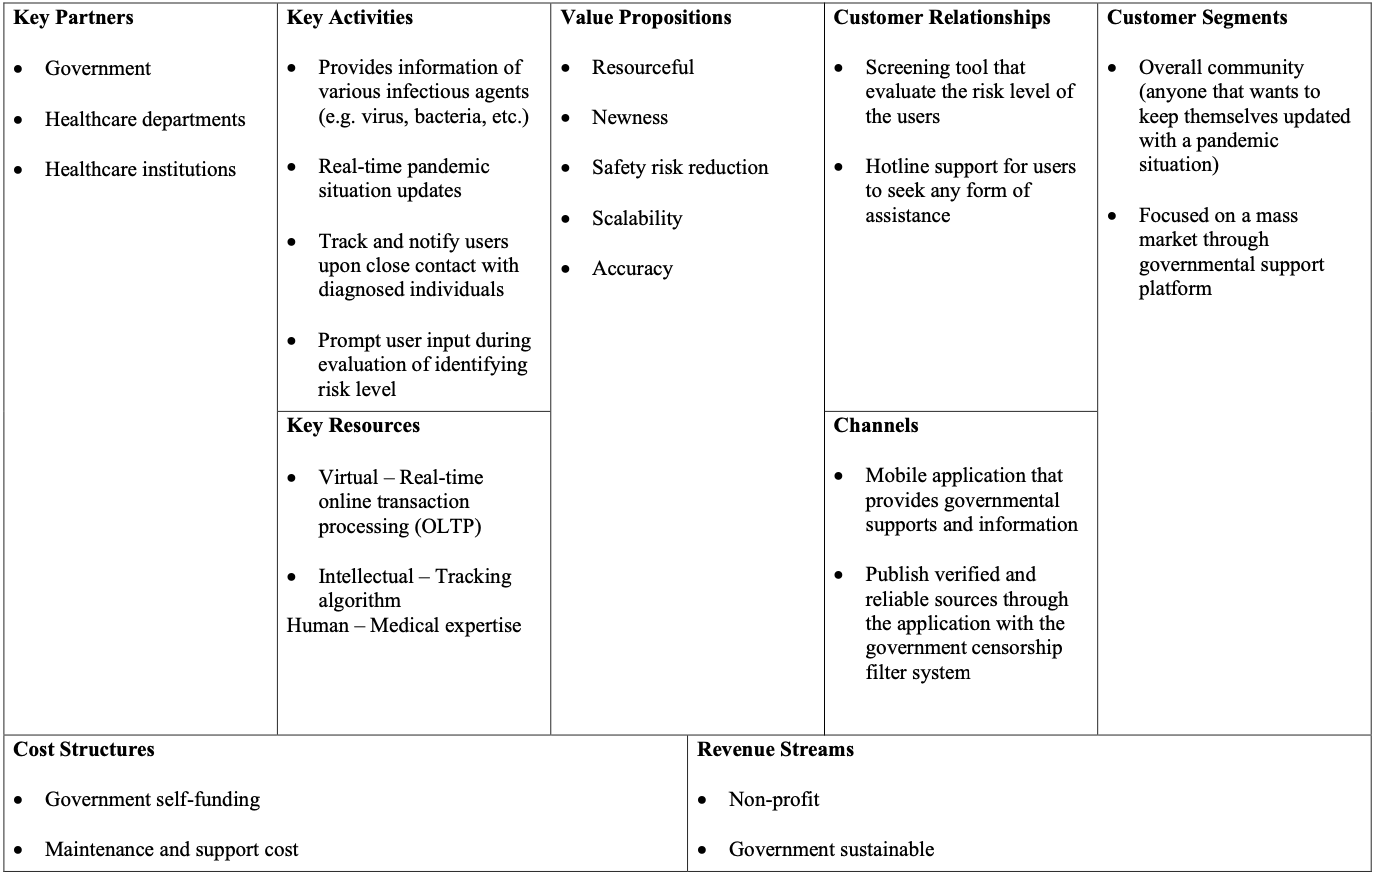
\includegraphics[width=21cm,angle=90,origin=c]{img/bmc.png}
        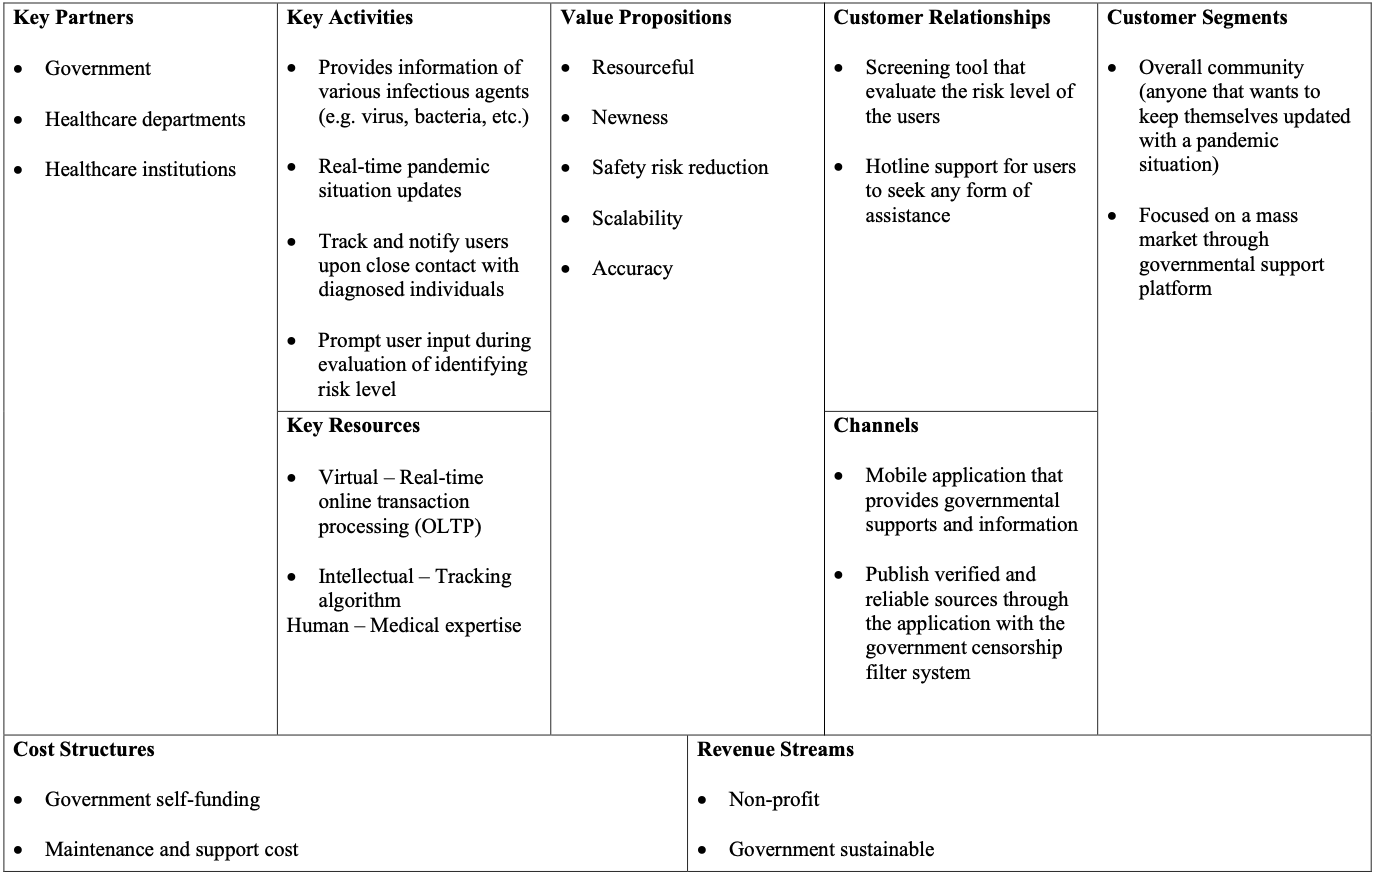
\includegraphics[width=\linewidth]{img/bmc.png}
        \caption{Business Model Canvas}
        \label{fig:bmc}
      \end{figure}
    
    \subsubsection{Paper prototyping}
      \par This approach is to provide a quick way to visualize the conceptual designs that could be a wireframe for the digital interfaces. A total of 9 simple interfaces of low-fidelity wireframes were created to showcase the general process of the possible solution.
      \begin{figure}[H]
        \centering
        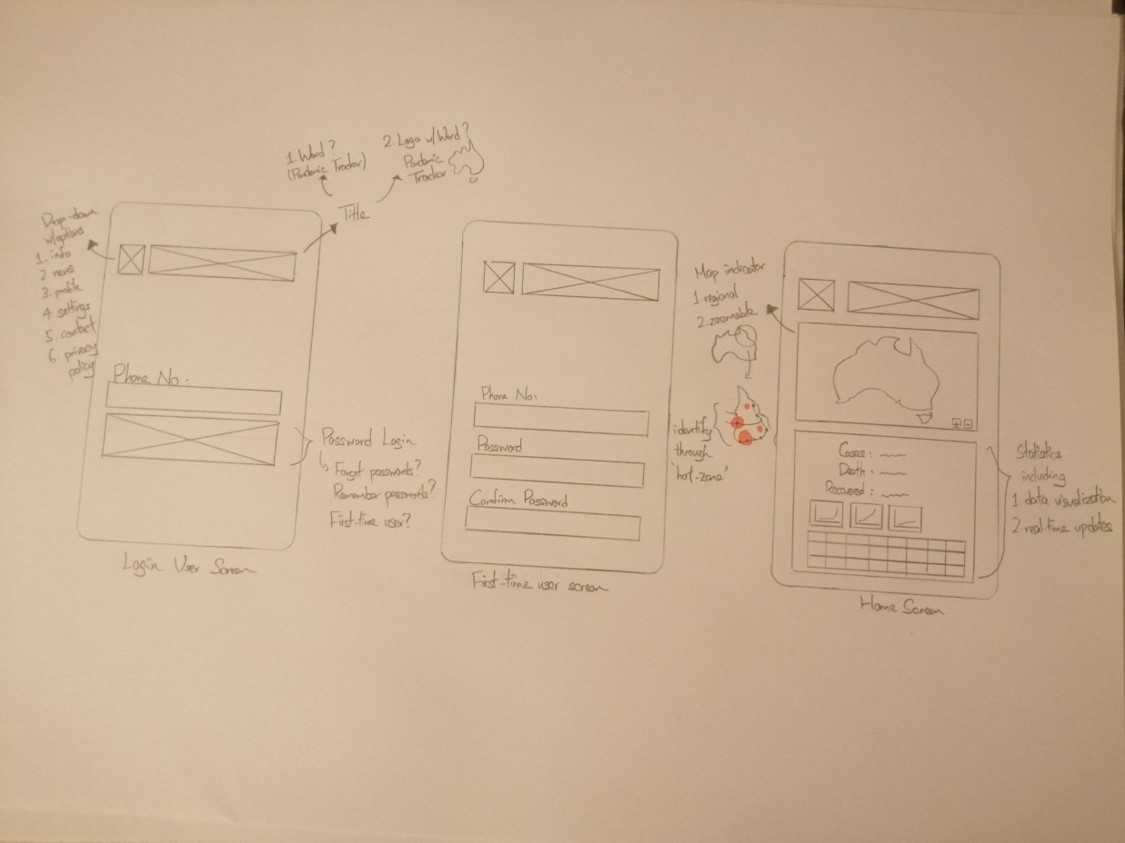
\includegraphics[width=\linewidth]{img/low-fidelity-prototype/sketch-1.png}
        \caption{Login, Register and Home Screen}
        \label{fig:prototype-01}
      \end{figure}
      
      \par Based on Figure \ref{fig:prototype-01}, the wireframe consists of the login, register and home screen interfaces, A valid phone number and a password is required for login. For first-time user, the login screen will have a link directing the user to the register screen to fill in the phone number and password to register as a member. Account recovery methods such as password reset will be included if the users forget their password. The home screen would include a heatmap indicator with statistical data of regional information including zone safety level, statistics, distribution of cases (orange dots in colour).
      
      \begin{figure}[H]
        \centering
        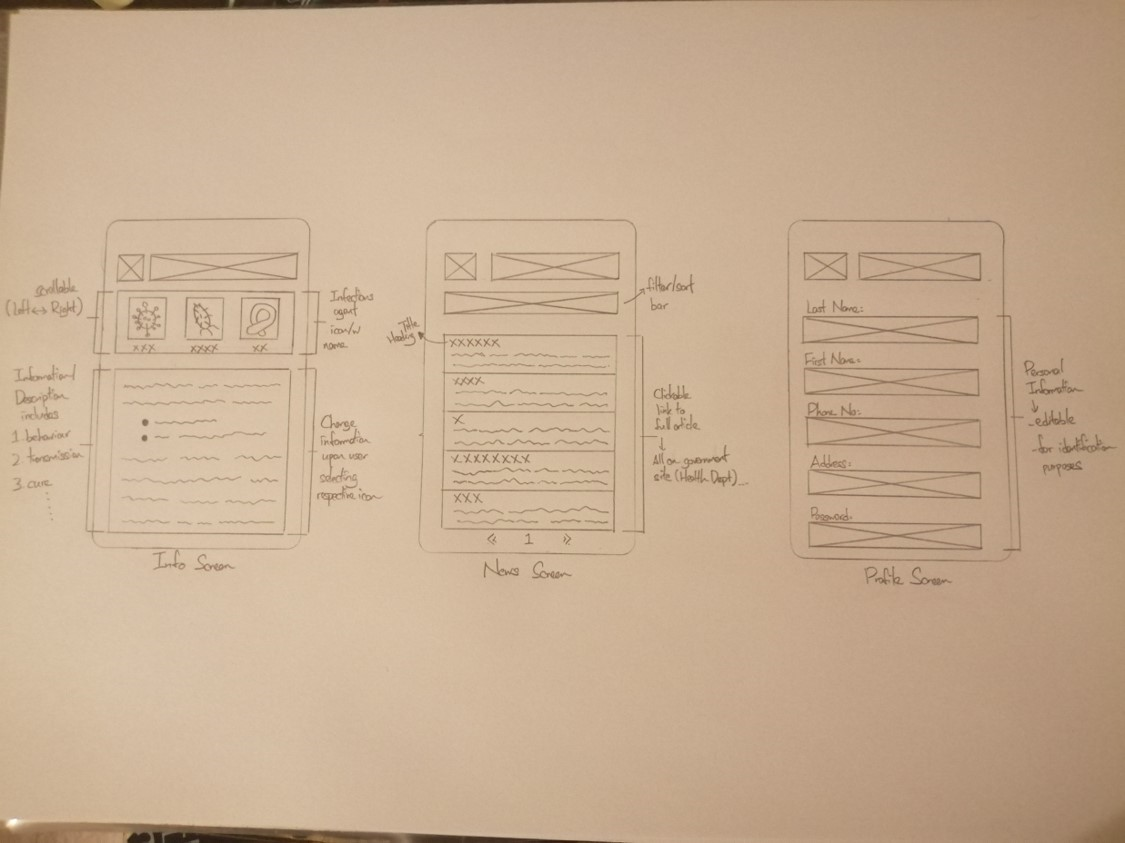
\includegraphics[width=\linewidth]{img/low-fidelity-prototype/sketch-2.png}
        \caption{Info, News and Profile Screen}
        \label{fig:prototype-02}
      \end{figure}

      \par Figure \ref{fig:prototype-02} shows the information, news and profile screen. Basic information of the infectious agents will be explained in layman terms which includes behaviour, characteristics, transmission and more. The following news screen are latest updated articles from verified publishers for any international and domestic news. The profile screen will display basic information consists of the authentic name of the user, phone no, and home address, which is crucial when immediate quarantine or government support is needed.

      \begin{figure}[H]
        \centering
        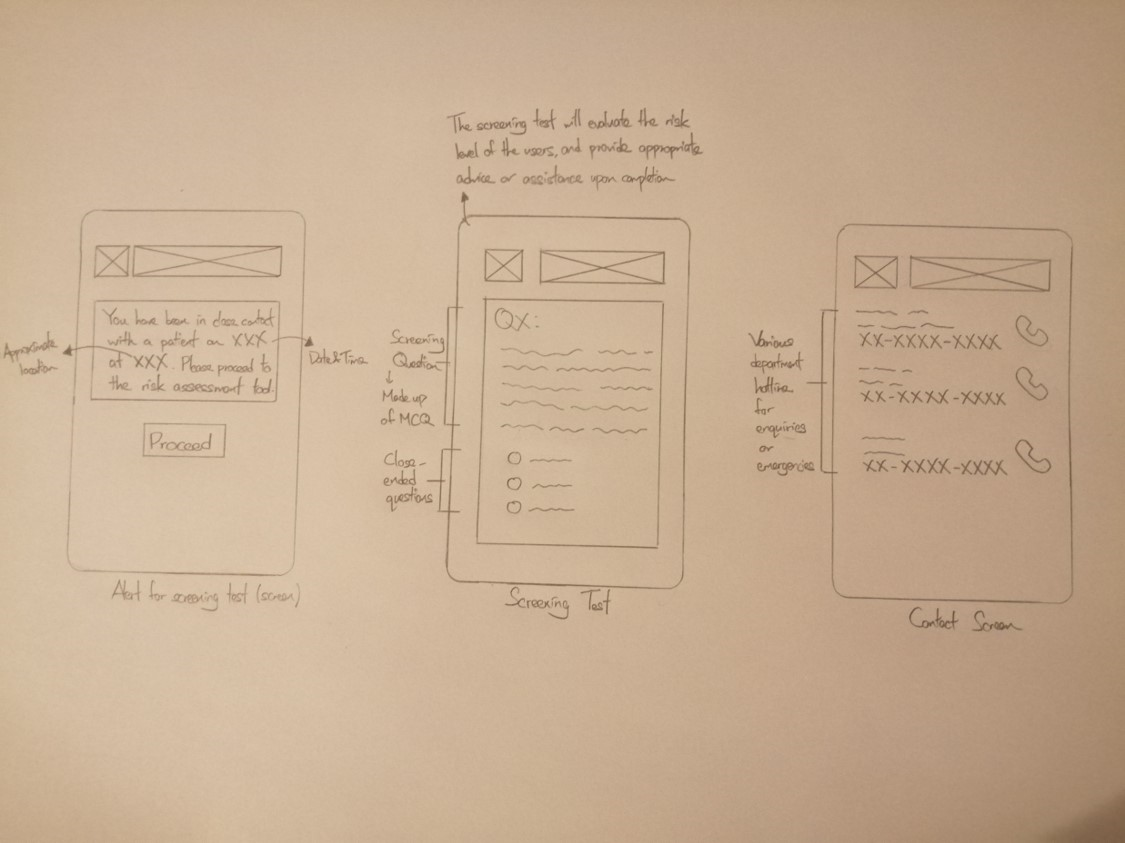
\includegraphics[width=\linewidth]{img/low-fidelity-prototype/sketch-3.png}
        \caption{Notification, Q\&A and Contact Screen}
        \label{fig:prototype-03}
      \end{figure}
      
      \par An alert notification, screening test and contact screen is shown in Figure \ref{fig:prototype-03}. The alert notification would pop up when the user has been verified having close contact with a diagnosed individual. The user will then be prompted to proceed to the Q\&A panel for a short evaluation. The result will display the user’s personal risk level, which may or may not necessarily to request medical support. Apart from this, the contact screen is listed with relevant government hotlines that could be helpful for enquiries or emergencies directly.

    \subsubsection{Digital Prototyping}
      \par This approach is to provide a high-fidelity sketch for multiple interfaces for interactive purposes. A wireframe is built upon a mixture of simulations and design mechanism. The current digital prototypes do not focus on the main functionalities of how a pandemic application should work, rather it focused on finding elements that could be included by studying user behaviour through usability testing to increase adoption and retention rate.

      \vspace{0.5cm}
      \par \textbf{Map Simulation}
      \vspace{0.5cm}
      \begin{figure}[H]
        \centering
        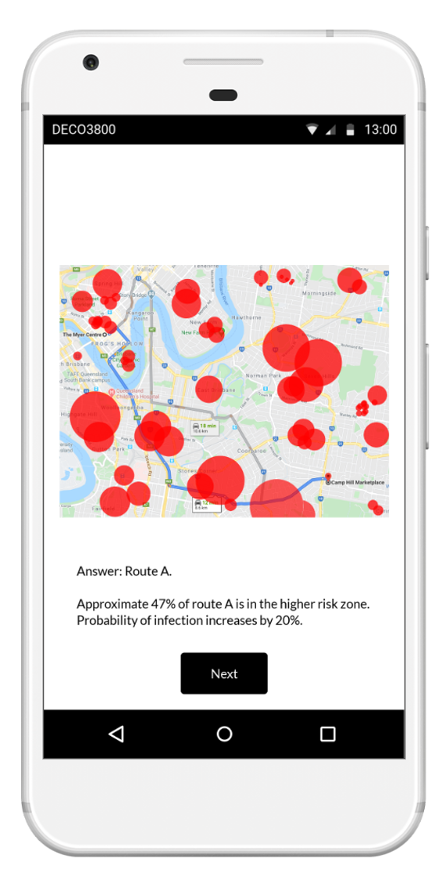
\includegraphics[scale=1]{img/digital-prototype/map-simulation.png}
        \caption{Map Simulation}
        \label{fig:digi-proto-01}
      \end{figure}
      \par The above Figure \ref{fig:digi-proto-01} simulation was proposed as a part of the product goals to improve decision making in risk assessment during travelling. Moreover, this simulation is integrated with the real-time heat map generated from the COVID-19 statistics. This algorithm will be included to calculate the user infection rate throughout the planned journey which happen to be in the hot zone when travelling.
      \par This simulation could act as a supplementary tool for helping user to make sound judgement to considers their surrounding loved ones as well. This could also invoke empathy among the users and therefore encourages it for journey planning. Thus, helping user to build a stronger relationship with their loved ones among this pandemic period.
      
      \vspace{0.5cm}
      \par \textbf{Quarantine Life Simulation}
      \vspace{0.5cm}
      \begin{figure}[H]
        \centering
        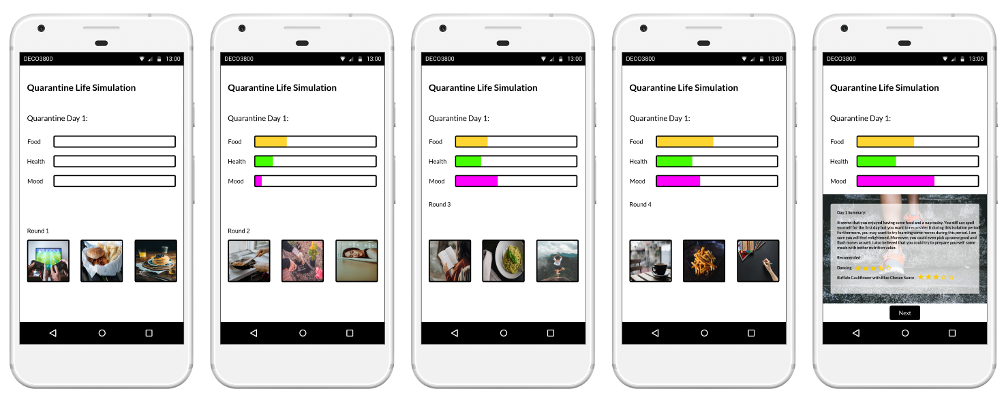
\includegraphics[scale=1]{img/digital-prototype/quarantine-life.png}
        \caption{Quarantine Life Simulation}
        \label{fig:digi-proto-02}
      \end{figure}
      \par The above Figure \ref{fig:digi-proto-02} simulation through cognitive learning was proposed as a part of the product goals to promote a healthier lifestyle during this pandemic period. Moreover, this simulation implemented via gamification through selecting a desire picture through each round daily. The food, health and mood barometers are each an attribute representation of eating habits, vitality and mental state. The system will then analyse the user behaviour and provide a summary according to the user selection including the total percentages in the barometers. The summary will include user the behavioural pattern and provide recommendations to improve certain attributes. Hence, this simulation could help encourages habits and behaviours change during this pandemic period for user to adopt a healthier lifestyle for low stress living.

  \subsection{Behavioral Design}
    \par Behavioural design is implemented for the purpose of increasing user adoption and retention rate. This is to ensure user would continuously interact with the application not merely for the main functionalities but also for sub-components through understanding user behaviour. Hence, we integrate the principles of behavioural design into our proposed solution.

    \subsubsection{Behavioral Modelling}
      \begin{figure}[H]
        \centering
        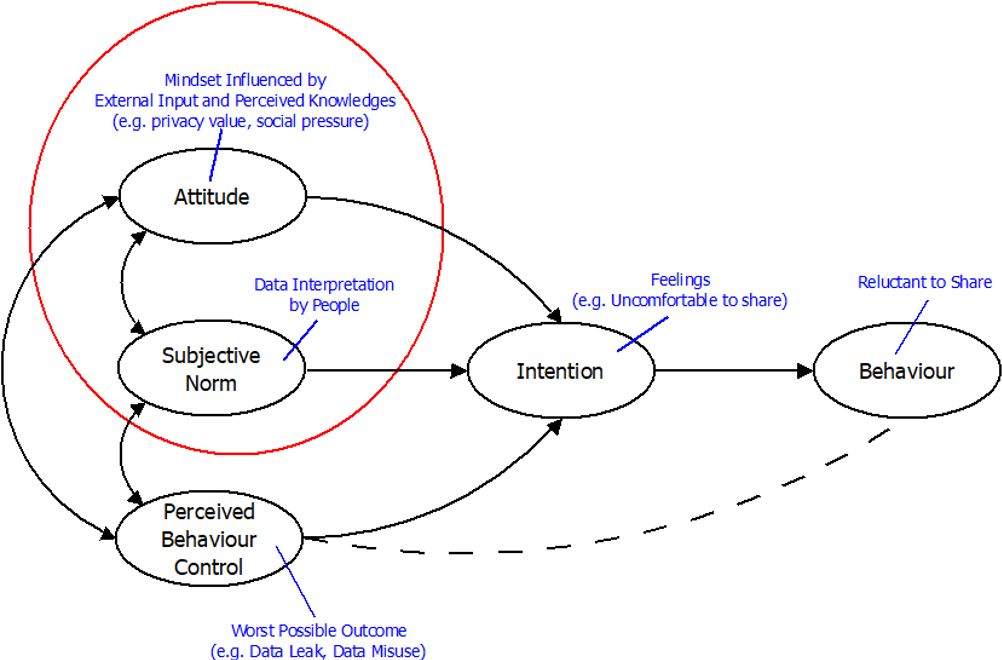
\includegraphics[scale=1]{img/digital-prototype/behavior-model.png}
        \caption{Data Sharing Behavior Model}
        \label{fig:behavior-model}
      \end{figure}
      \par This modelling concept template is borrowed from \parencite{Ian8}. The above Figure \ref{fig:behavior-model} shows the modelling with my notation on how data privacy has been perceived by the general public now. For the current public behaviour for launched pandemic mobile application, most of them are reluctant to share their data and does not find it really helpful. This are mostly affected by how they perceived the worst possible outcome interpreted by the public or based on their knowledge. Hence, it may further influence their perspective collectively known as collective consciousness. This may however create norms that are misleading through social pressure for other people as well. Hence, we would like implements some behaviour design principles to change people’s attitude not creating or affected subjective norms (red circle shown above).
    
    \subsubsection{Example}
      \begin{figure}[H]
        \centering
        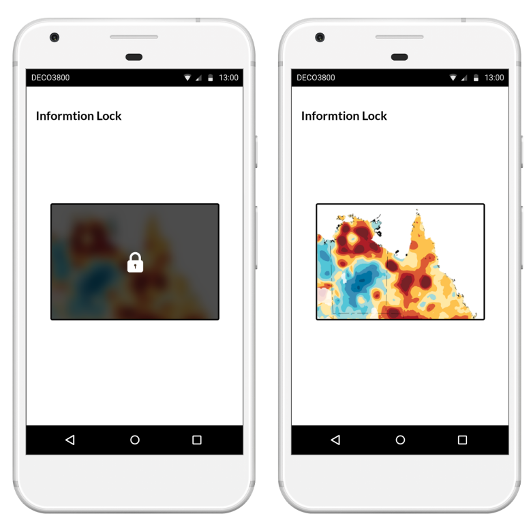
\includegraphics[scale=1]{img/digital-prototype/info-lock-screen.png}
        \caption{Information Lock Screen}
        \label{fig:digi-proto-03}
      \end{figure}
      \par From the above Figure \ref{fig:digi-proto-03}, it displayed the Queensland regional heatmap for COVID-19 zones. The information on left is lock while unlocked on the right. This design applied a concept called sequential information release. This approach is to limit the disclosure of sensitive data and information to the application users. Moreover, it is equally important and fair to all users when certain users are providing necessary information while others are taking for granted. In such case, we do not imply consent to any users who are unwilling to share their information while also protecting the privacy of other users who share their information. Thus, it promotes a scenario of user inducing altruistic behaviour known as reciprocal altruism. In other words, we study the user psychology to create guidelines to implement behaviour design principles to increase user experience that could positively affect the society by not creating social pressure.

  \subsection{Usability Testing}
    \par The purpose of usability testing is to evaluate a product through the prototype based on the feedbacks collected from users. It helps refining user requirement and visual design of the product throughout the development cycle. Moreover, it focused on how users interact with the prototype, completing the given tasks, and observe their behaviour during testing. It could collect valuable insights through learning the user’s behaviour and preference from the prototype. Thus, the insights could further improve the prototype for each testing.
    \par The prototypes used for testing session are the map simulator and quarantine life simulator. All the participants joined have given their consent for the testing session.
    
    \subsubsection{Retrospective Think Aloud (RTA)}
      \par This technique requires participants to retrace their steps when the session is complete. This technique is particularly useful to verbalize participants thoughts and embed the process into their memory. Hence, it could check whether the participants could visualize the content during memory tracing, which indicates how the visual content is delivered to them during the session. In other word, the user preferences and behaviours would influence on the values and core process they perceived with the simulation prototype demos.
      \par Findings:
      \begin{itemize}
        \item Map Simulator:
          \begin{itemize}
            \item 4 of 5 participants thinks that the information is insufficient for convincing them from leaving the house.
            \item All participants do not remember the major hot zones after answering it.
          \end{itemize}
        \item Quarantine Life Simulation:
          \begin{itemize}
            \item 3 of 5 participants spent a longer average time testing the quarantine life simulator.
            \item 3 of 5 participants thinks that the quarantine life simulator is a fun-to-play game only.
          \end{itemize}
      \end{itemize}
    
    \subsubsection{Concurrent Probing}
      \par This testing technique requires participants to work on tasks and asking follow-up questions when the participant engaged uniquely within the session. This technique is suitable to prompt real-time feedbacks on upon each task executed, which could directly project their current feelings towards the prototypes. In other words, we could understand the user psychology path when carrying out tasks through how the application may evoke different feelings towards the user or the user behaviour in performing task on the application. Hence, it creates a minimum threshold on how these elements could provide its usefulness in increasing user retention rate through a MVP product.
      \par Findings:
        \begin{itemize}
          \item Map Simulator:
            \begin{itemize}
              \item All members suggested for more travel options. 
              \item 3 of 5 participants suggested to include information as hint when they think it is good and easy to reference for authentication.
            \end{itemize}
          \item Quarantine Life Simulation:
            \begin{itemize}
              \item 2 of 5 participants thinks that the selection rounds could be increase for a more thorough representation of their daily lifestyle.
              \item 4 of 5 participants thinks that the selection categories for each round in the quarantine life simulator are inconsistent. 
            \end{itemize}
        \end{itemize}

    \subsubsection{Insight Summary}
      \begin{itemize}
        \item Map Simulator:
          \begin{itemize}
            \item More useful statistical inputs are required to increase user interest and authenticity from verified sources. 
            \item Participants are likely wanting to travel in their own preferred transport only, which the current simulator only display one option travelling by car only. In other words, this may happen to due habits issue or lack of confidence travelling with non-preferred vehicle during this period.
            \item Create important visual components to be more appealing and attractive for developing as a semantic memory during memory encoding (Behavioural design principles).
            \item Providing minor support as guidelines such as nudge could its memory point for user impression.
          \end{itemize}
        \item Quarantine Life Simulation:
          \begin{itemize}
            \item Create selection within the category in each round for better memory tracing.
            \item Providing selection pictures that are more approximate to local culture and habits accordingly.
            \item More in-depth analysis for the daily summary should be carried out with the prompted input.
            \item Participants tends to spend more time for recalling and retracing memory with the selection pictures each round, indicating the significant values as an additional component to increase retention rate.
          \end{itemize}
      \end{itemize}

  
      